%\documentstyle[10pt,twoside]{article}
%\documentstyle[twoside]{article}
\documentclass[twoside]{article}
\setlength{\oddsidemargin}{0.25 in}
\setlength{\evensidemargin}{-0.25 in}
\setlength{\topmargin}{-0.6 in}
\setlength{\textwidth}{6.5 in}
\setlength{\textheight}{8.5 in}
\setlength{\headsep}{0.75 in}
\setlength{\parindent}{0 in}
\setlength{\parskip}{0.1 in}

\usepackage{graphicx}
\usepackage{url}

%
% The following commands sets up the lecnum (lecture number)
% counter and make various numbering schemes work relative
% to the lecture number.
%
\newcounter{lecnum}
\renewcommand{\thepage}{\thelecnum-\arabic{page}}
\renewcommand{\thesection}{\thelecnum.\arabic{section}}
\renewcommand{\theequation}{\thelecnum.\arabic{equation}}
\renewcommand{\thefigure}{\thelecnum.\arabic{figure}}
\renewcommand{\thetable}{\thelecnum.\arabic{table}}
\newcommand{\dnl}{\mbox{}\par}

%
% The following macro is used to generate the header.
%
\newcommand{\lecture}[4]{
   \pagestyle{myheadings}
   \thispagestyle{plain}
   \newpage
   \setcounter{lecnum}{#1}
   \setcounter{page}{1}
   \noindent
   \begin{center}
   \framebox{
      \vbox{\vspace{2mm}
    \hbox to 6.28in { {\bf CMPSCI~677~~~Distributed~\&~Operating Systems
                        \hfill Spring 2019} }
       \vspace{4mm}
       \hbox to 6.28in { {\Large \hfill Lecture #1: #2  \hfill} }
       \vspace{2mm}
       \hbox to 6.28in { {\it Lecturer: #3 \hfill Scribe: #4} }
      \vspace{2mm}}
   }
   \end{center}
   \markboth{Lecture #1: #2}{Lecture #1: #2}
   \vspace*{4mm}
}

%
% Convention for citations is authors' initials followed by the year.
% For example, to cite a paper by Leighton and Maggs you would type
% \cite{LM89}, and to cite a paper by Strassen you would type \cite{S69}.
% (To avoid bibliography problems, for now we redefine the \cite command.)
%
\renewcommand{\cite}[1]{[#1]}

% \input{epsf}

%Use this command for a figure; it puts a figure in wherever you want it.
%usage: \fig{NUMBER}{FIGURE-SIZE}{CAPTION}{FILENAME}
\newcommand{\fig}[4]{
            %\vspace{0.2 in}
            \centerline{\includegraphics[scale=#2]{#4}}
            \begin{center}
            Figure \thelecnum.#1:~#3
            \end{center}
    }

% Use these for theorems, lemmas, proofs, etc.
\newtheorem{theorem}{Theorem}[lecnum]
\newtheorem{lemma}[theorem]{Lemma}
\newtheorem{proposition}[theorem]{Proposition}
\newtheorem{claim}[theorem]{Claim}
\newtheorem{corollary}[theorem]{Corollary}
\newtheorem{definition}[theorem]{Definition}
\newenvironment{proof}{{\bf Proof:}}{\hfill\rule{2mm}{2mm}}

% Some useful equation alignment commands, borrowed from TeX
\makeatletter
\def\eqalign#1{\,\vcenter{\openup\jot\m@th
  \ialign{\strut\hfil$\displaystyle{##}$&$\displaystyle{{}##}$\hfil
      \crcr#1\crcr}}\,}
\def\eqalignno#1{\displ@y \tabskip\@centering
  \halign to\displaywidth{\hfil$\displaystyle{##}$\tabskip\z@skip
    &$\displaystyle{{}##}$\hfil\tabskip\@centering
    &\llap{$##$}\tabskip\z@skip\crcr
    #1\crcr}}
\def\leqalignno#1{\displ@y \tabskip\@centering
  \halign to\displaywidth{\hfil$\displaystyle{##}$\tabskip\z@skip
    &$\displaystyle{{}##}$\hfil\tabskip\@centering
    &\kern-\displaywidth\rlap{$##$}\tabskip\displaywidth\crcr
    #1\crcr}}
\makeatother

% **** IF YOU WANT TO DEFINE ADDITIONAL MACROS FOR YOURSELF, PUT THEM HERE:



% Some general latex examples and examples making use of the
% macros follow.

\begin{document}

%FILL IN THE RIGHT INFO.
%\lecture{**LECTURE-NUMBER**}{**DATE**}{**LECTURER**}{**SCRIBE**}
\lecture{21}{April 24}{Prashant Shenoy}{\textbf{}}


\section{Distributed File Systems (DFS)}
A DFS is a file system where files are stored on multiple distributed machines.
\subsection{Coda}
Coda is a research FS designed at CMU. It was designed to support Mobile devices. It was \textbf{disconnection transparent} which means users would see the all files even if the system was temporarily disconnected. The FS proactively cache files that user is accessing so that in case of disconnection, user can still work on the local copy of the file. It may also happen that a user is disconnected and they try to access a file that is not cached in which case they will know that they are disconnected. The cache adapts so that only files that the user wants are cached. Some source control systems also work this way.


\begin{figure}[htbp]
\centering
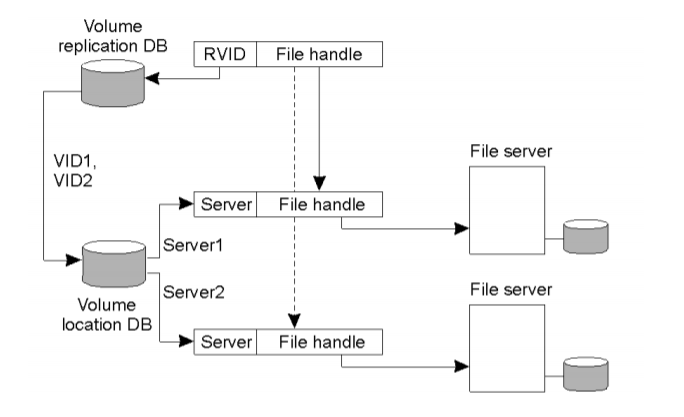
\includegraphics[width=6in]{Figures/codaarch.png}
\caption{Coda architecture} \label{fig:codaarch}
\end{figure}



Each directory can be replicated on multiple servers. Each file in Coda belongs to exactly one volume. A volume may be replicated across several servers as shown in Figure \ref{fig:codaarch}. Multiple logical (replicated) volumes map to the same
physical volume. Any file identifier is of length $96$ bits which consists of $32$ bit RVID and $64$ bit file handle. 

\subsubsection{Issues with server replication}
\begin{figure}[htbp]
\centering
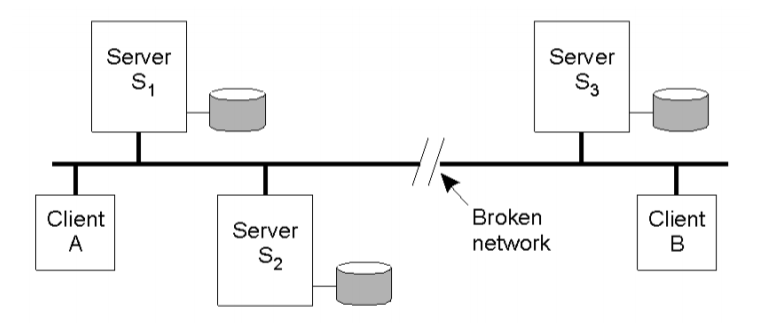
\includegraphics[width=6in]{Figures/serv_rep.png}
\caption{Server replication issues in Coda} \label{fig:serv_rep}
\end{figure}
Figure \ref{fig:serv_rep} shows what happens when there is a disconnection in the network. Each partition uses the local cached copies and application treat the local cached copies as actual files and all operations are performed on them. Later, when the network reconnects, the two parts resynchronize. Each file has a version vector which is a vector containing versions of the file on all other servers. This is incremented by each server when the file is updated locally. When all servers are synchronized all elements of the version vector will be the same. However, they will be different in case of disconnections. During reconnection, if a version vector of a server 1 is strictly greater than server 3, then server 1 has the latest copy. If server 1 and 2 has version vector [2,2,1] and server 3 has vector [1,1,2] then there is no strict ordering in which case there will be a write-write conflict and there needs to be a manual merge conflict.

\begin{figure}[htbp]
\centering
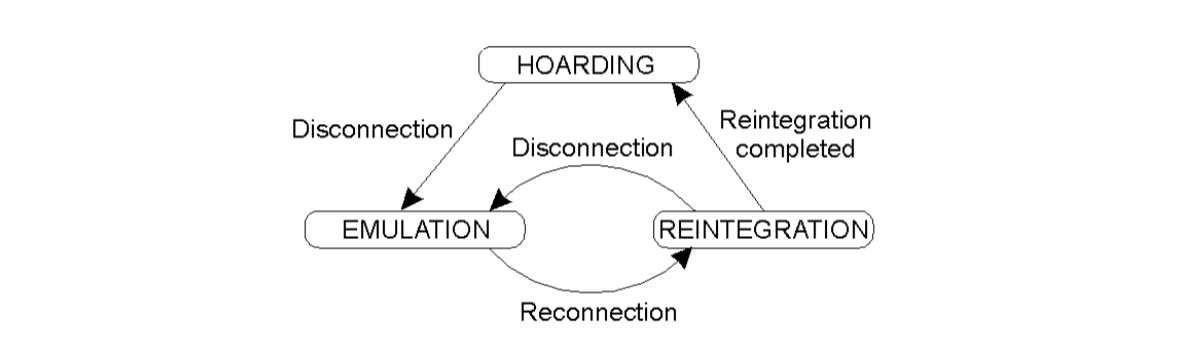
\includegraphics[width=6in]{Figures/disc_oper.png}
\caption{Disconnected operation in Coda} \label{fig:disc_oper}
\end{figure}
% FIGURE NUMBER
Figure \ref{fig:disc_oper} shows the state-transition diagram of a Coda client with respect to a volume. It has $3$ states: HOARDING, EMULATION and REINTEGRATION. Whenever the client is connected to the network, it is in HOARDING mode. In this mode, the client does aggressive caching. Whenever the client is disconnected, it makes a transition into the EMULATION mode. In this mode, all the file requests are serviced by the local cache and the version vectors get updated. The local cache file acts just like the actual file. On reconnection, the client goes to the REINTEGRATION mode. Resynchronization and version vector comparisons are made in this mode.


\subsubsection{Transactional Semantics}
Coda treats all operations as transactions which entails serializability, ACID properties etc. This is important since there are frequent disconnections and there could be conflicts on resynchronization.

\subsubsection{Client Caching}
Conda ensures cache consistency using callbacks which is a  type of server-push consistency. Any update to a file by a client is sent to all other clients so the clients update their caches.


\subsection{xFS (No Server FS)}
This is a decentralized serverless file system. So there are no explicit servers and clients. Nodes can be both servers and clients. The resources are shared by all nodes. So instead of fetching data from a server, nodes have to find where a particular piece of data is located and then fetch it. An example of what the nodes look like is shown in Figure \ref{fig:xfsarch}
\begin{figure}[htbp]
\centering
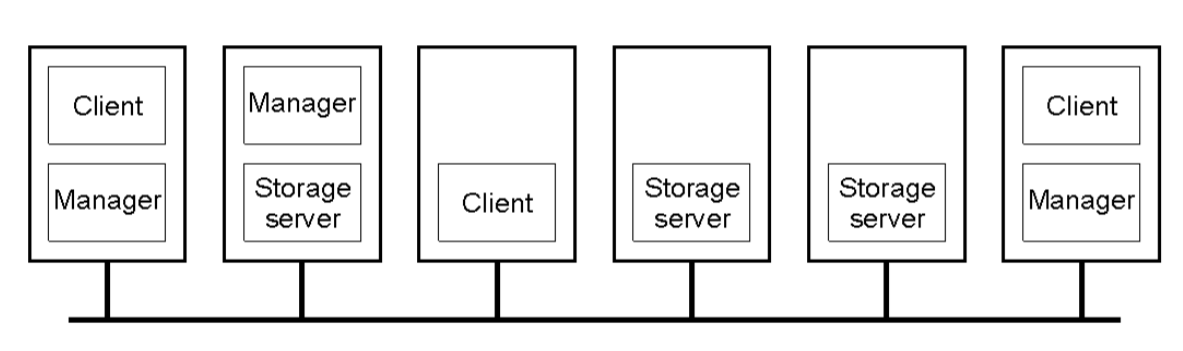
\includegraphics[width=6in]{Figures/xfsarch.png}
\caption{An example of nodes in xFS} \label{fig:xfsarch}
\end{figure}

xFS is built on two fundamental file systems: RAID and Log-structured File System as explained below.

\subsubsection{RAID}
RAID stands for Redundant Array of Independent Disks. In RAID based storage,  files are striped across multiple disks. Disk failures are to be handled explicitly in case of a RAID based storage. Fault tolerance is built through redundancy. 

\begin{figure}[htbp]
\centering
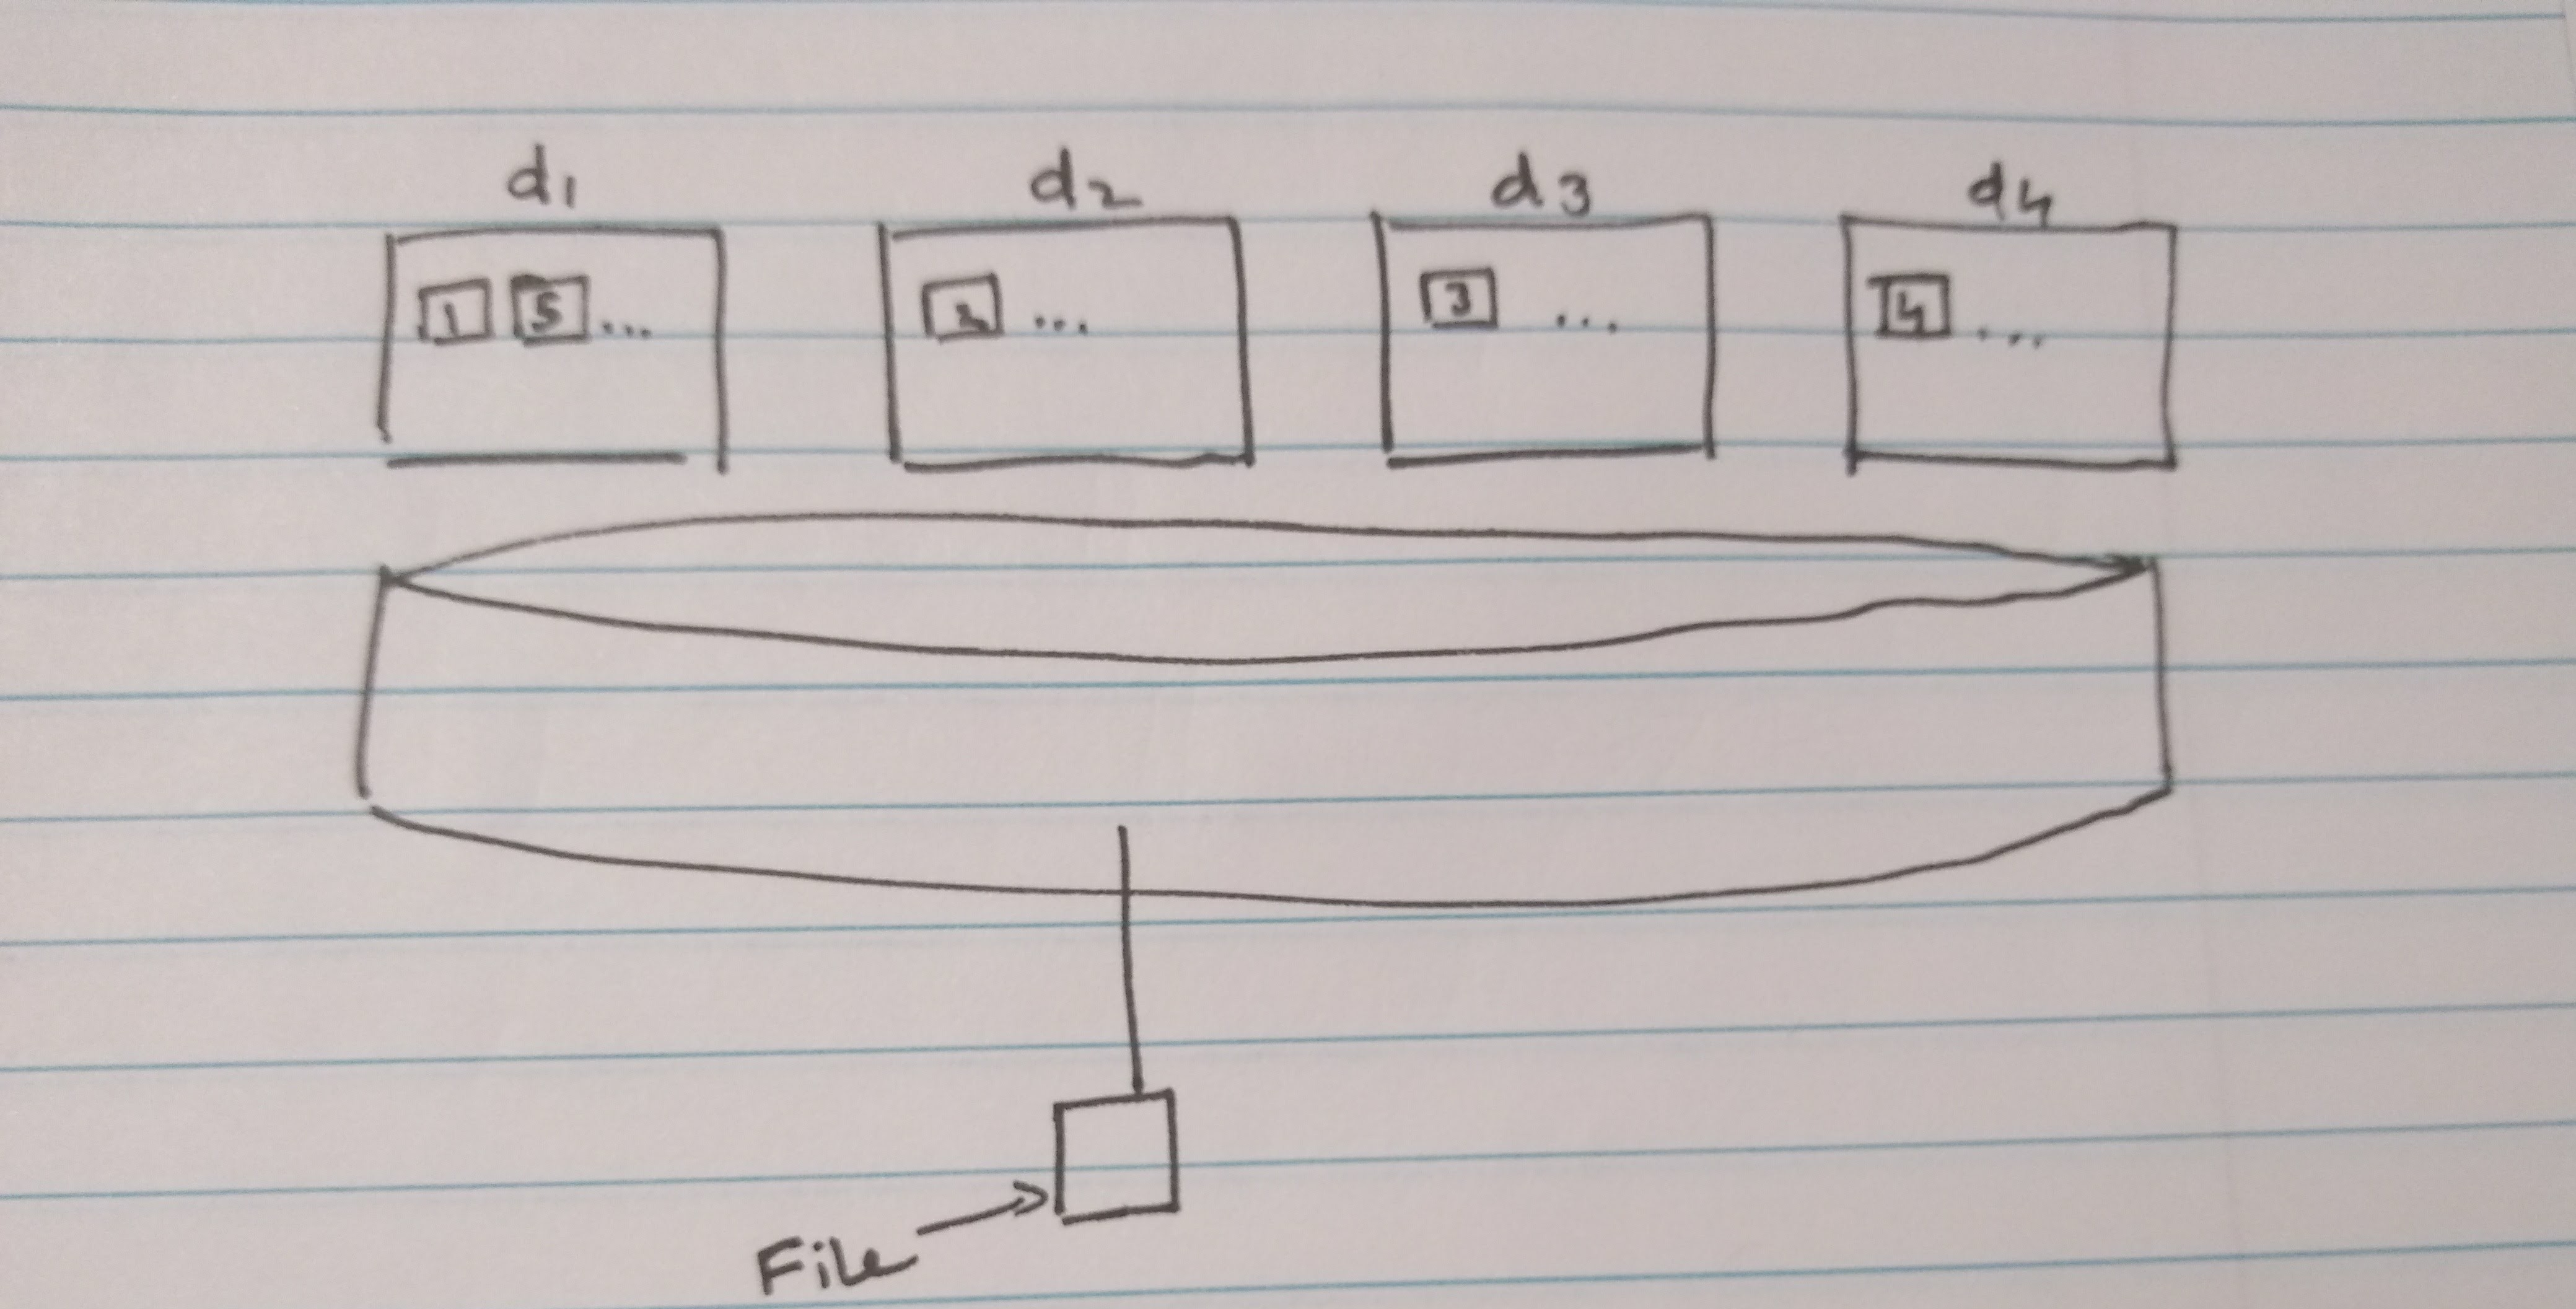
\includegraphics[width=6in]{Figures/striping.jpg}
\caption{Striping in RAID} \label{fig:striping}
\end{figure}
Figure \ref{fig:striping} shows how files are stored in RAID. d1,...d4 are disks. Each file is divided into blocks and stored in the disks in a round robin fashion. So if a disk fails, all parts stored on that disk are lost. It has an advantage that file can be read in parallel because data is stored on multiple disks and they can be read at the same time. Secondly, storage is load balanced. If a file is popular and is requested more often, the load is evenly balanced across nodes. This also results in higher throughput.


A disadvantage of striping is failure of disks. The performance of this system depends on the reliability of disks. A typical disk lasts for 50,000 hours which is also knows as the Disk MTTF. As we add disks to the system, the MTTF drops as disk failures are independent.\\

$\textrm{Reliability of N disks} = \textrm{Reliability of 1 disk} \div N$

We implement some form of redundancy in the system to avoid disadvantages caused by disk failures. Depending on the type of redundancy the system can be classified into different groups:

\subsubsection{RAID 1 (Mirroring)}
From figure \ref{fig:RAID1}, we can see that in RAID 1 each disk is fully duplicated. Each logical write involves two physical writes. This scheme is not cost effective as it involves a 100\% capacity overhead.
\begin{figure}[htbp]
\centering
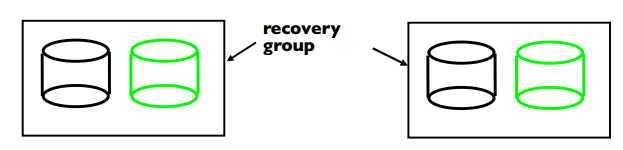
\includegraphics[width=4in]{Figures/mirroring.png}
\caption{RAID 1} \label{fig:RAID1}
\end{figure}

\subsubsection{RAID 4}
\begin{figure}[htbp]
\centering
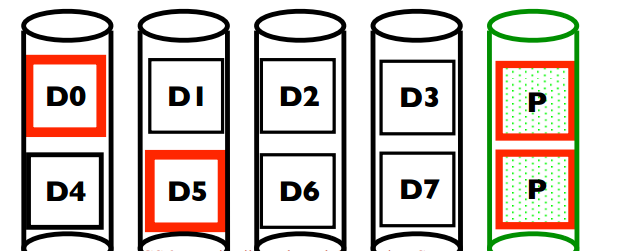
\includegraphics[width=4in]{Figures/RAID4.png}
\caption{RAID 4} \label{fig:RAID4}
\end{figure}
This method uses parity property to construct \texttt{ECC} (Error Correcting Codes) as shown in Figure \ref{fig:RAID4}. First a parity block is constructed from the existing blocks. Suppose the blocks $D_0$, $D_1$, $D_2$ and $D_3$ are striped across $4$ disks. A fifth block (parity block) is constructed as:
\begin{equation}
P = D_0 \oplus D_1 \oplus D_2 \oplus D_3 \nonumber
\end{equation}
If any disk fails, then the corresponding block can be reconstructed using parity. For example:
\begin{equation}
D_0 =  D_1 \oplus D_2 \oplus D_3 \oplus P \nonumber
\end{equation}

This error correcting scheme is one fault tolerant. Only one disk failure can be handled using RAID 4. The size of parity group should be tuned so as there is low chance of more than 1 disk failing in a single parity group.


\subsubsection{RAID 5}
\begin{figure}[htbp]
\centering
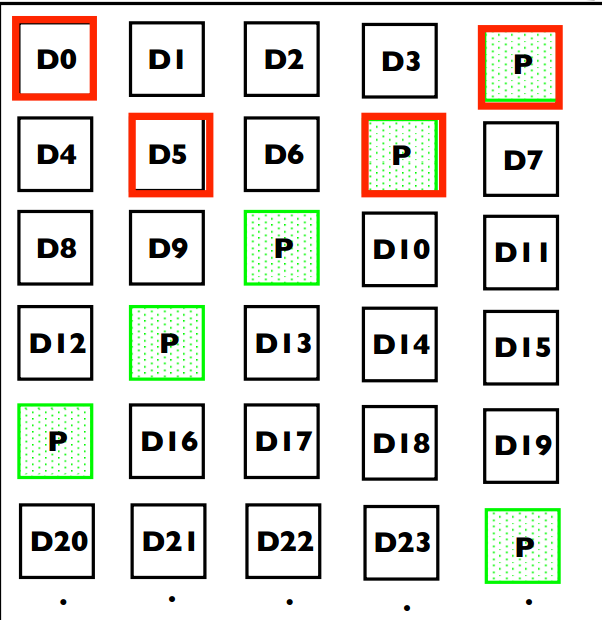
\includegraphics[width=4in]{Figures/RAID5.png}
\caption{RAID 5} \label{fig:RAID5}
\end{figure}
One of the main drawbacks of RAID 4 is that all parity blocks are stored on the same disk. Also, there are k + 1 I/O operations on each small write, where k is size of the parity block. Moreover, load on the parity disk is sum of load on other disks in the parity block. This will saturate the parity disk and slow down entire system.

In order to overcome this issue, RAID 5 uses distributed parity as shown in Figure \ref{fig:RAID5}. The parity blocks are distributed in an interleaved fashion.

Note: All RAID solutions have some write performance impact. There is no read performance impact.

RAID implementations are mostly on hardware level. Hardware RAID implementation are much faster than software RAID implementations.

\subsubsection{Log-Structured FS (LFS)}
Purpose of LFS is to write data as a structured log. We keep appending blocks on disks as we do in a log file. This results in a very high write throughput.

In practice, we use a memory cache to increase efficiency as I/O operations on disks takes time. However, due to this cache, the traffic seen by the disks are predominantly writes, and few reads (caused by cache misses). Hence, we can optimize disks for write traffic. This is the idea behind LFS.

In LFS, we keep on writing sequentially. This minimizes seek time for a magnetic disk, hence increases the throughput. If a read comes after a write, we have to seek the block to be read which decreases the performance. Therefore, LFS works well if the I/O operations are mostly writes.

This advantage is only for magnetic disks and is not for SSDs, as there are no moving parts. SSDs provides random access.

In LFS, when we update a block, we write a new block, and mark the previous block as garbage. So a disadvantage of LFS is that we have to do garbage collection, which requires seek overheads. Also, it makes meta-data management complicated, as we have to update file Inode every time we update a block.

\subsubsection{xFS and RAID}
xFS uses software RAID by having multiple disks across multiple machines over a network. Small writes are expensive since updating a single block results in updating the parity which requires reading of all the other data blocks.

Moreover, xFS writes data using LFS. xFS implements striping which gives parallelism, RAID which gives fault-tolerance, and LFS wich provides high write throughput.


\subsection{HDFS}
Hadoop Distributed File System (HDFS) is used for processing very large datasets. 
HDFS files system has following goals:
\begin{itemize}
\item Fault-tolerant -  System needs fault tolerant disks to store the large datasets.
\item Streaming Data access - FS should provide batch processing rather than interactive usage.
\item Size of the datasets are very large.
\item Typically datasets are going to see WORM workloads. Which mean Write Once Read Many. This is because datasets are created only once, and is not changed afterwards, and only read many times.
\item As the size of datasets are too large, we prefer moving computation instead of data.
\end{itemize}

\begin{figure}[htbp]
\centering
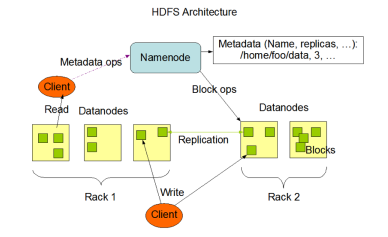
\includegraphics[width=4in]{Figures/HDFS.png}
\label{fig:HDFS}
\end{figure}

HDFS uses large block size of around 64MB (Typical FS has 4KB block). Normally, files are much larger than block size, and large block size helps in reducing the seek overhead.

HDFS does not use RAID, but simply replicates every file 3 times (default value) and stored on random machines. This is a 2-fault tolerant system.

In fig \ref{fig:HDFS}, we have meta data nodes which keep information about the datanodes. 

\subsection{GFS}
Google File Systems is similar to HDFS. Each file is replicated on 3 different machines. A metadata nodes contains index of physical machines that stores a file. 

File chunks are stored on standard linux files system. These have large block sizes which are tracked by GFS.

\subsection{S3}
There are storage systems which store a objects instead of a file. In object files system, we have key (hash of object) against which the object is mapped. 

S3 also doesn't uses RAID. It replicates objects across data center. Moreover, there is no naming scheme like a FS. Storage is flat. And we are required to use HTTP to query required objects.
\end{document}
